\documentclass[12pt]{article}


\usepackage{amssymb}
\usepackage{amsmath}
\usepackage{fullpage}
\usepackage{epsfig}
\usepackage{epstopdf, hyperref, xcolor}
\everymath{\displaystyle}
\usepackage{enumerate}

\newif\ifans

\anstrue

\begin{document}

\begin{center}
\underline{\LARGE{Parametric Equations, Tangent Lines, \& Arc Length}}
\end{center}

\noindent SUGGESTED REFERENCE MATERIAL:

\bigskip

\noindent As you work through the problems listed below, you should reference Chapter 10.1 of the recommended textbook (or the equivalent chapter in your alternative textbook/online resource) and your lecture notes.

\bigskip

\noindent EXPECTED SKILLS:

\begin{itemize}

\item Be able to sketch a parametric curve by eliminating the parameter, and indicate the orientation of the curve. 

\item Given a curve and an orientation, know how to find parametric equations that generate the curve. 

\item Without eliminating the parameter, be able to find $\frac{dy}{dx}$ and $\frac{d^2y}{dx^2}$ at a given point on a parametric curve.

\item Be able to find the arc length of a smooth curve in the plane described parametrically.

\end{itemize}

\noindent PRACTICE PROBLEMS:

\medskip

\noindent {\bf For problems 1-5, sketch the curve by eliminating the parameter.  Indicate the direction of increasing $t$.}

\begin{enumerate}

\item $\left\{\begin{array}{l}
x=2t+3\\
y=3t-4\\
0\leq t \leq 3 \end{array}\right.$

\ifans{\fbox{\parbox{1\linewidth}{\begin{center}
$y=\frac{3}{2}x-\frac{17}{2}$ from $(3,-4)$ to $(9,5)$\\
\medskip
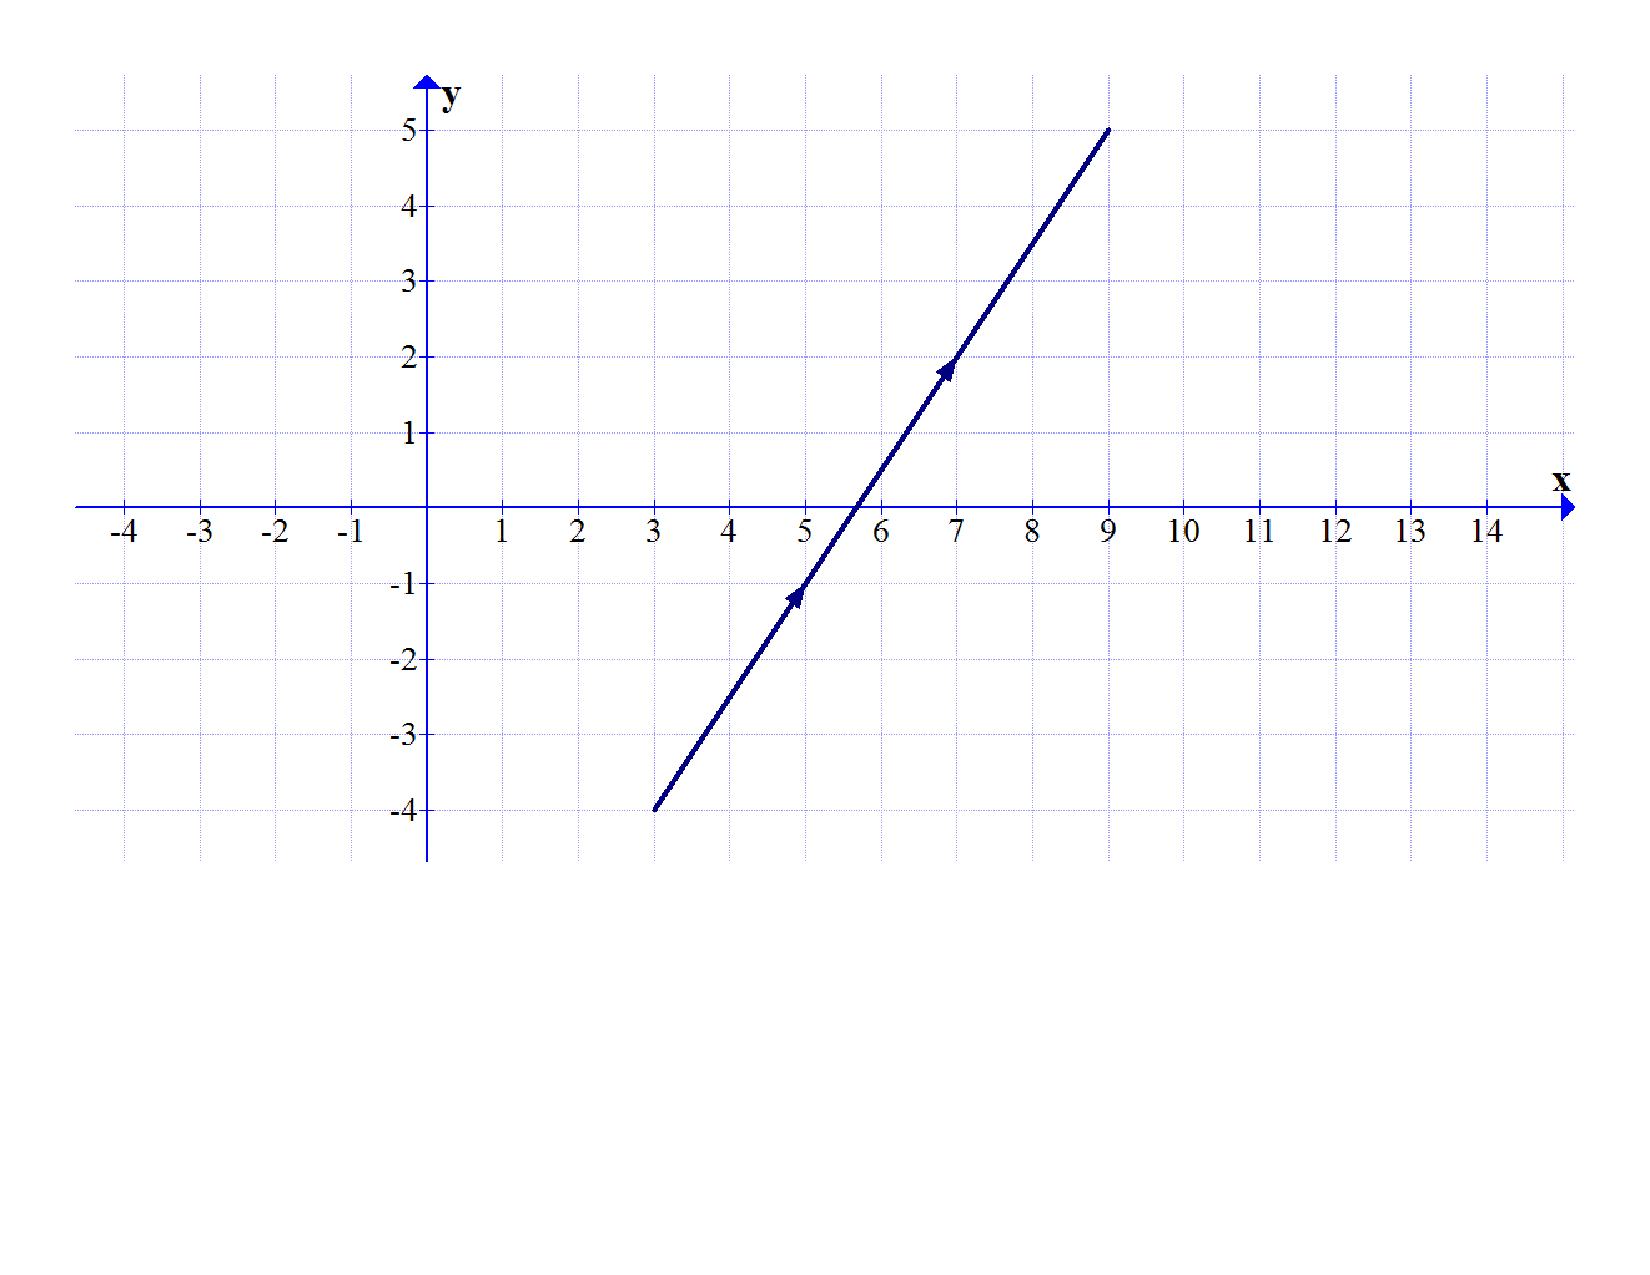
\includegraphics[scale=0.3]{ans1.pdf}
\end{center}}}} \fi

\item $\left\{\begin{array}{l}
x=2\cos{t}\\
y=3\sin{t}\\
\pi \leq t \leq 2\pi \end{array}\right.$ 

\ifans{\fbox{\parbox{1\linewidth}{\begin{center}$\frac{x^2}{4}+\frac{y^2}{9}=1$ from $(-2,0)$ to $(2,0)$\\
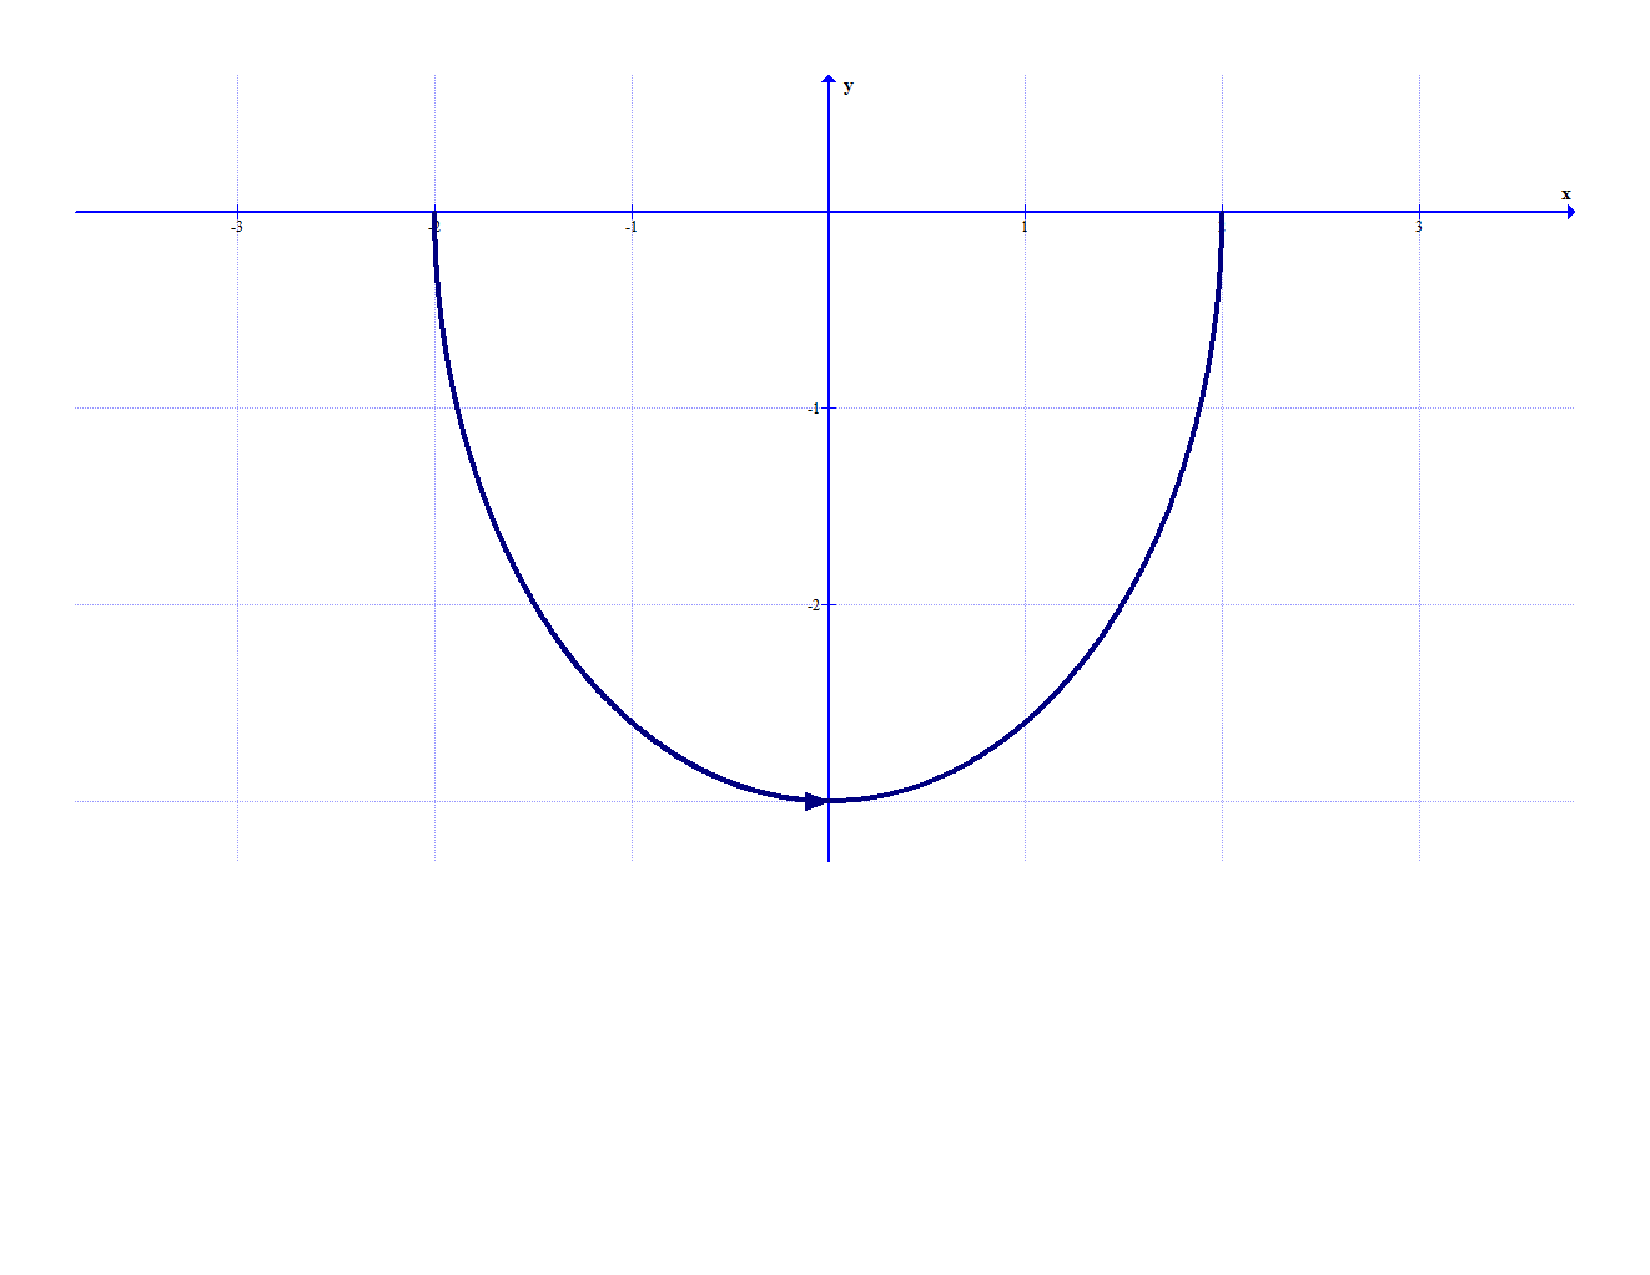
\includegraphics[scale=0.25]{ans2.pdf}
\end{center}}}} \fi

\item $\left\{\begin{array}{l}
x=t-5\\
y= \sqrt{t}\\
0 \leq t \leq 9\end{array}\right.$ 

\ifans{\fbox{\parbox{1\linewidth}{\begin{center}$y=\sqrt{x+5}$ from $(-5,0)$ to $(4,3)$\\
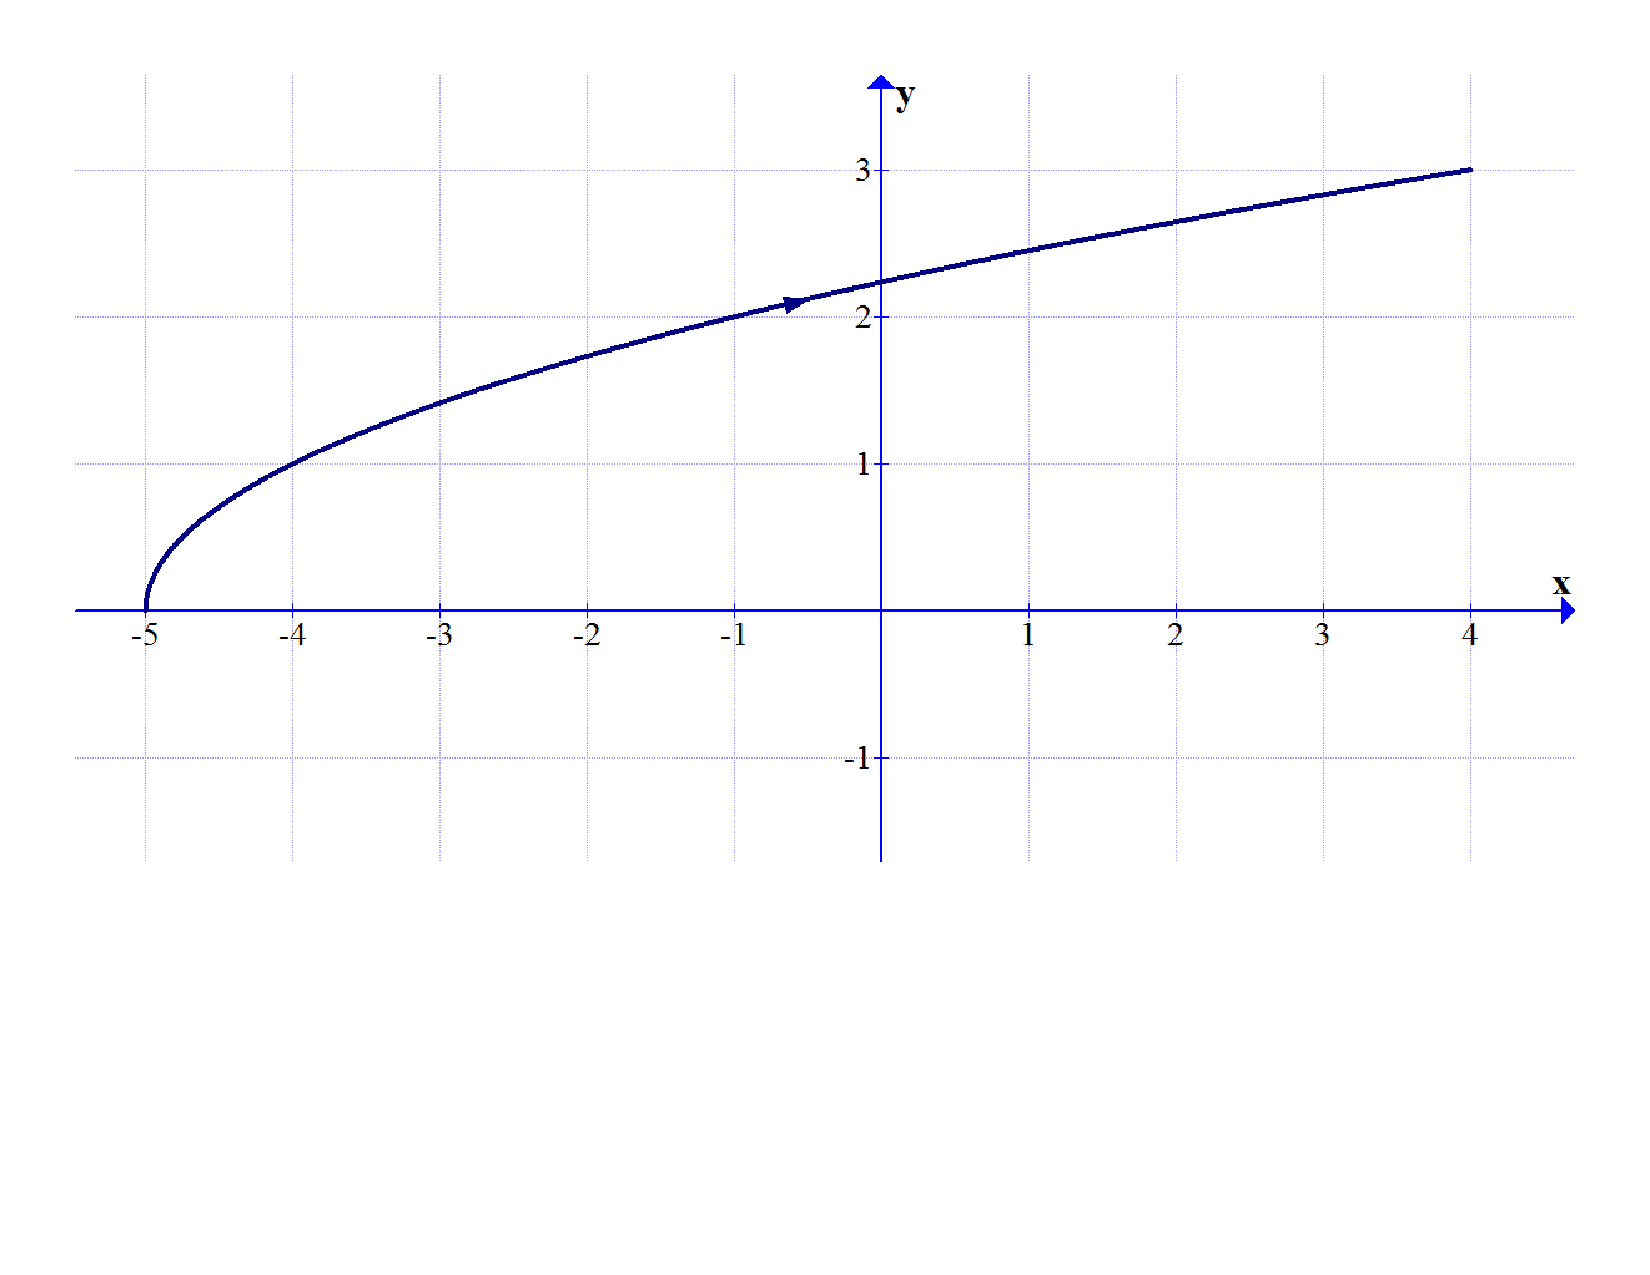
\includegraphics[scale=0.25]{ans3.pdf}
\end{center}}}} \fi

\item $\left\{\begin{array}{l}
x=\sec{t}\\
y=\tan^2{t}\\
0 \leq t < \frac{\pi}{2} \end{array} \right.$

\ifans{\fbox{\parbox{1\linewidth}{\begin{center}
$y=x^2-1$ for $x \geq 1$\\
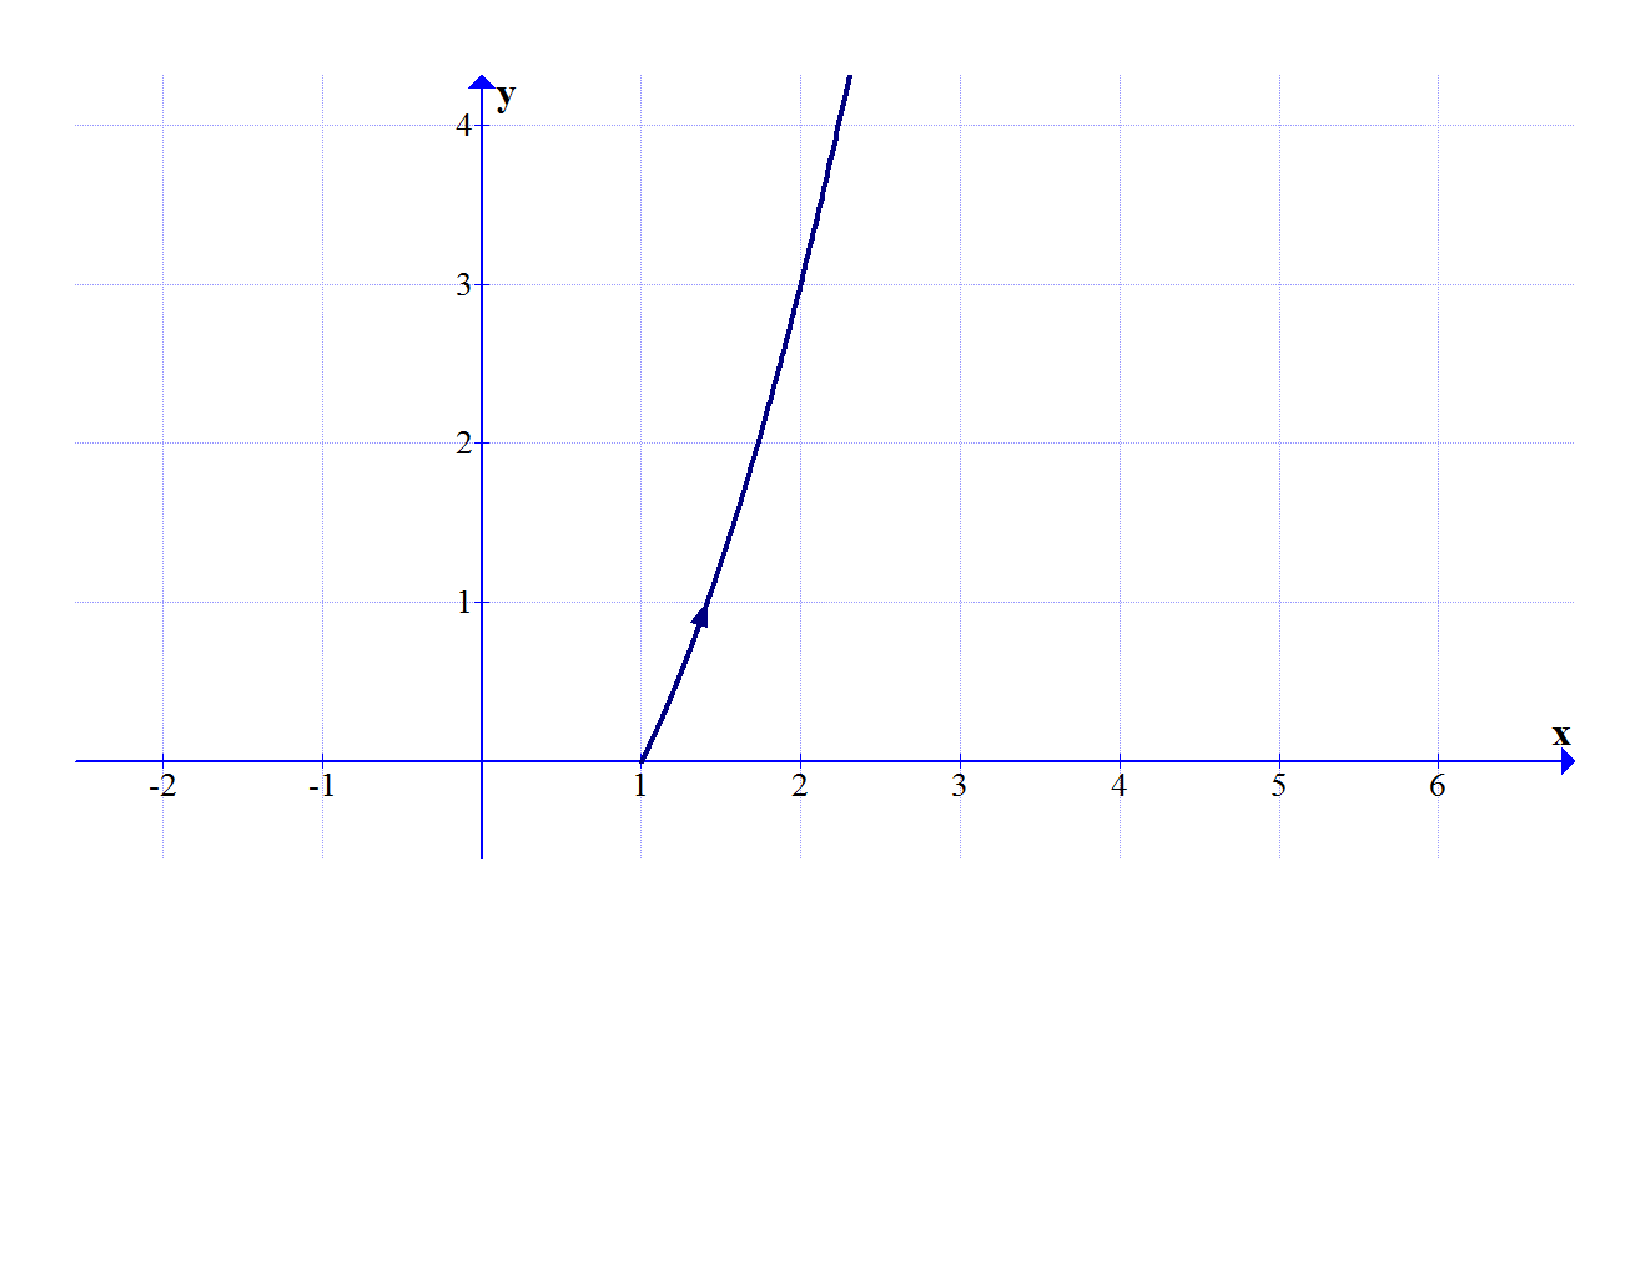
\includegraphics[scale=0.25]{ans4.pdf}
\end{center}}}} \fi

\item $\left\{\begin{array}{l}
x=\sin{t}\\
y=\cos{(2t)}\\
-\frac{\pi}{2} \leq t \leq \frac{\pi}{2} \end{array} \right.$

\ifans{\fbox{\parbox{1\linewidth}{\begin{center}
$y=1-2x^2$ from $(-1,-1)$ to $(1,-1)$\\
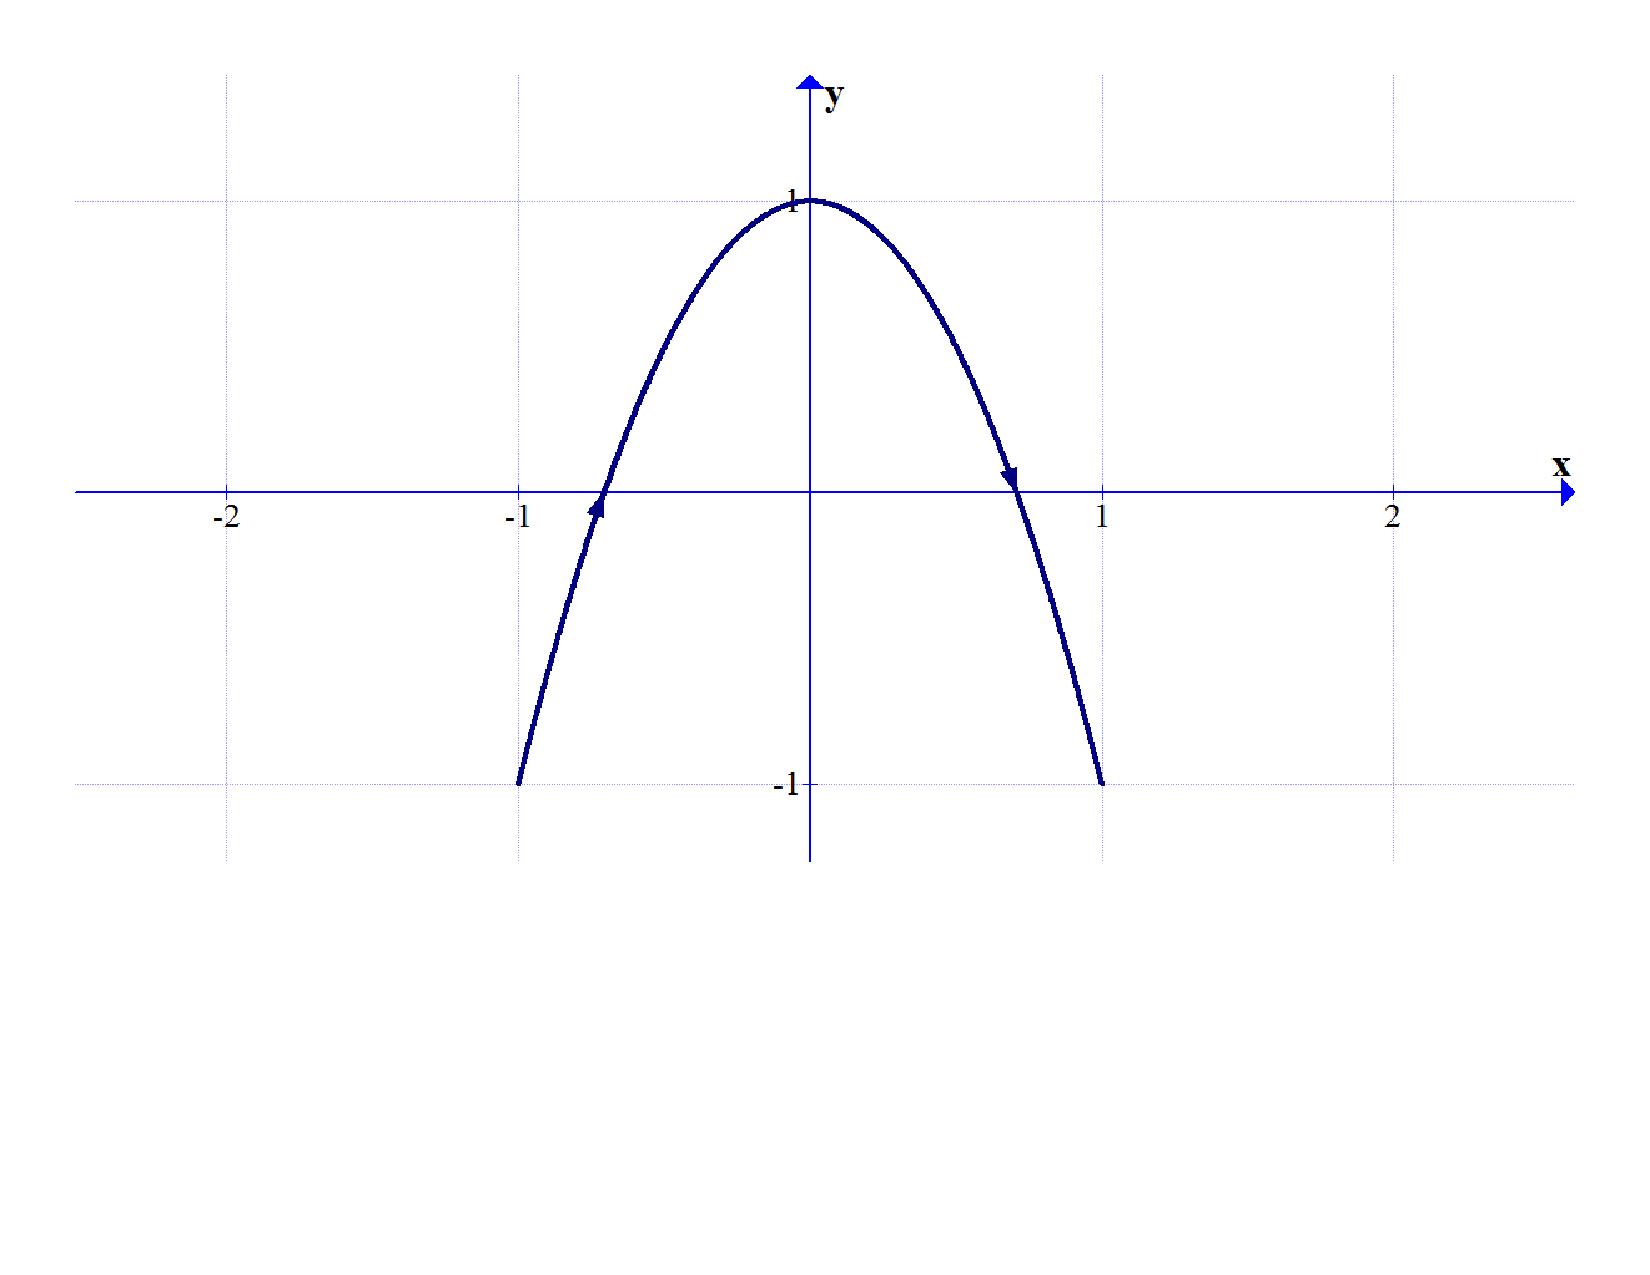
\includegraphics[scale=0.25]{ans5.pdf}\end{center}}}} \fi

\end{enumerate}

\noindent {\bf For problems 6-10, find parametric equations for the given curve. (For each, there are many correct answers; only one is provided.)}

\begin{enumerate}
\setcounter{enumi}{5}

\item A horizontal line which intersects the y-axis at $y=2$ and is oriented rightward from $(-1,2)$ to $(1,2)$. 

\ifans{\fbox{$\left\{\begin{array}{l}
x=t\\
y=2\\
-1\leq t\leq 1\end{array}\right.$}} \fi

\item A circle or radius 4 centered at the origin, oriented clockwise.  

\ifans{\fbox{$\left\{\begin{array}{l}
x=4\sin{t}\\
y=4\cos{t}\\
0\leq t\leq 2\pi\end{array}\right.$}} \fi

\item A circle of radius 5 centered at $(1,-2)$, oriented counter-clockwise. 

\ifans{\fbox{$\left\{\begin{array}{l}
x=5\cos{t}+1\\
y=5\sin{t}-2\\
0\leq t\leq 2\pi \end{array}\right.$; Detailed Solution: \textcolor{blue}{\href{http://www.math.drexel.edu/classes/Calculus/resources/Math122HW/Solutions/122_17_Parametric_08.pdf}{Here}} }} \fi

\item The portion of $y=x^3$ from $(-1,-1)$ to $(2,8)$, oriented upward. 

\ifans{\fbox{$\left\{\begin{array}{l}
x=t\\
y=t^3\\
-1\leq t\leq 2\end{array}\right.$}} \fi

\newpage

\item The ellipse $\frac{x^2}{4}+\frac{y^2}{16}=1$, oriented counter-clockwise. 

\ifans{\fbox{$\left\{\begin{array}{l}
x=2\cos{t}\\
y=4\sin{t}\\
0\leq t\leq 2\pi\end{array}\right.$}} \fi

\end{enumerate}

\noindent {\bf For problems 11-13, find $\frac{dy}{dx}$ and $\frac{d^2y}{dx^2}$ at the given point without eliminating the parameter.}

\begin{enumerate}
\setcounter{enumi}{10}

\item The curve $\left\{\begin{array}{l}
x=3\sin{(3t)}\\
y=\cos{(3t)}\\
0<t<2\pi\end{array}\right.$ at $t=\pi$ 

\ifans{\fbox{$\left.\frac{dy}{dx}\right|_{t=\pi}=0$; $\left.\frac{d^2y}{dx^2}\right|_{t=\pi}=\frac{1}{9}$}} \fi

\item The curve $\left\{\begin{array}{l}
x=t^2\\
y=3t-2\\
t \geq 0 \end{array}\right.$ at $t=1$ 

\ifans{\fbox{$\left.\frac{dy}{dx}\right|_{t=1}=\frac{3}{2}$; $\left.\frac{d^2y}{dx^2}\right|_{t=1}=-\frac{3}{4}$}} \fi

\item The curve $\left\{\begin{array}{l}
x=2\tan{t}\\
y=\sec{t}\\
0 \leq t \leq \frac{\pi}{3} \end{array}\right.$ at $t=\frac{\pi}{4}$ 

\ifans{\fbox{$\left.\frac{dy}{dx}\right|_{t=\pi/4}=\frac{\sqrt{2}}{4}$, $\left.\frac{d^2y}{dx^2}\right|_{t=\pi/4}=\frac{\sqrt{2}}{16}$; Detailed Solution: \textcolor{blue}{\href{http://www.math.drexel.edu/classes/Calculus/resources/Math122HW/Solutions/122_17_Parametric_13.pdf}{Here}}}} \fi

\item Consider the curve described parametrically by $\left\{\begin{array}{l}
x=\sqrt{t}\\
y=\sqrt[3]{t}+1\\
t \geq 0 \end{array}\right.$

\begin{enumerate}

\item Compute $\left.\frac{dy}{dx}\right|_{t=64}$ without eliminating the parameter.

\ifans{\fbox{$\left.\frac{dy}{dx}\right|_{t=64}=\frac{1}{3}$}} \fi

\newpage

\item Eliminate the parameter and verify your answer for part (a) using techniques from differential calculus.

\ifans{\fbox{\parbox{1\linewidth}{The curve is equivalent to $y=x^{2/3}+1$, $x \geq 0$.  And, $t=64$ corresponds to $x=8$.  Thus, $\left.\frac{dy}{dx}\right|_{t=64}=\left.\frac{dy}{dx}\right|_{x=8}=\frac{1}{3}$}}} \fi

\item Compute an equation of the line which is tangent to the curve at the point corresponding to $t=64$.

\ifans{\fbox{$y-5=\frac{1}{3}(x-8)$}} \fi

\end{enumerate}

\item Consider the curve described parametrically by $\left\{\begin{array}{l}
x=2\cos{t}\\
y=4\sin{t}\\
0 \leq t \leq 2\pi \end{array}\right.$

\begin{enumerate}

\item Compute $\left.\frac{dy}{dx}\right|_{t=\pi/4}$ without eliminating the parameter.

\ifans{\fbox{$\left.\frac{dy}{dx}\right|_{t=\pi/4}=-2$}} \fi

\item Eliminate the parameter and verify your answer for part (a) using techniques from differential calculus.

\ifans{\fbox{\parbox{1\linewidth}{The curve is equivalent to the ellipse $\frac{x^2}{4}+\frac{y^2}{16}=1$.  And, $t=\frac{\pi}{4}$ corresponds to the point $(x,y)=(\sqrt{2},2\sqrt{2})$.  Thus, you can use implicit differentiation and $\left.\frac{dy}{dx}\right|_{t=\pi/4}=\left.\frac{dy}{dx}\right|_{(x,y)=\left(\sqrt{2},2\sqrt{2}\right)}=-2$}}} \fi

\item Compute an equation of the line which is tangent to the curve at the point corresponding to $t=\frac{\pi}{4}$.

\ifans{\fbox{$y-2\sqrt{2}=-2\left(x-\sqrt{2}\right)$}} \fi

\item At which value(s) of $t$ will the tangent line to the curve be horizontal?

\ifans{\fbox{$t=\frac{\pi}{2}$ and $t=\frac{3\pi}{2}$}} \fi

\end{enumerate}

\end{enumerate}

\noindent {\bf For problems 16-18, compute the length of the given parametric curve.}

\begin{enumerate}
\setcounter{enumi}{15}

\item The curve described by $\left\{\begin{array}{l}
x=t\\
\\
y=\frac{2}{3}t^{3/2}\\
\\
0 \leq t \leq 4 \end{array}\right.$

\ifans{\fbox{$-\frac{2}{3}+\frac{10\sqrt{5}}{3}$}} \fi

\item The curve described by $\left\{\begin{array}{l}
x=e^t\\
\\
y=\frac{2}{3}e^{3t/2}\\
\\
\ln{2} \leq t \leq \ln{3} \end{array}\right.$

\ifans{\fbox{$-2\sqrt{3}+\frac{16}{3}$; Detailed Solution: \textcolor{blue}{\href{http://www.math.drexel.edu/classes/Calculus/resources/Math122HW/Solutions/122_17_Parametric_17.pdf}{Here}}}} \fi

\item The curve described by $\left\{\begin{array}{l}
x=\frac{1}{2}t^2\\
\\
y=\frac{1}{3}t^3\\
\\
0 \leq t \leq \sqrt{3} \end{array} \right.$

\ifans{\fbox{$\frac{7}{3}$}} \fi

\item Compute the lengths of the following two curves:

\begin{center}
\begin{tabular}{cc}
$C_1(t)=\left\{\begin{array}{l}
x=\cos{t}\\
y=\sin{t}\\
0 \leq t \leq 2\pi \end{array} \right.$ \hspace{0.5 cm}& \hspace{0.5 cm}
$C_2(t)=\left\{\begin{array}{l}
x=\cos{(3t)}\\
y=\sin{(3t)}\\
0 \leq t \leq 2\pi \end{array} \right.$
\end{tabular}
\end{center}

Explain why the lengths are not equal even though both curves coincide with the unit circle.

\ifans{\fbox{\parbox{1\linewidth}{The length of $C_1(t)$ is $2\pi$ and the length of $C_2(t)=6\pi$.  Notice that $C_2(t)$ is the just curve $C_1(t)$ traversed three times.}}} \fi

\item This problem describes how you can find the area between a parametrically defined curve and the $x$-axis.\\

{\bf The Main Idea:} Recall that if $y=f(x)\geq 0$, then the area between the curve and the $x$-axis on the interval $[a,b]$ is $\int_a^b f(x)dx=\int_a^b y\,dx$.  Now, suppose that the same curve is described parametrically by $x=x(t)$, $y=y(t)$ for $t_0 \leq t \leq t_1$ and that the curve is traversed exactly once on this interval.  Then, $A=\int_a^b y\,dx=\int_{t_0}^{t_1} y(t)x^{\prime}(t)\,dt$.  \\

Consider the curve $\left\{\begin{array}{l}
x=\sin{t}\\
y=\cos{(2t)}\\
-\frac{\pi}{4} \leq t \leq \frac{\pi}{4} \end{array} \right.$

\begin{enumerate}

\item Compute the area between the graph of the given curve and the $x$-axis by evaluating $A=\int_{t_0}^{t_1} y(t)x^{\prime}(t) \,dt$.

\ifans{\fbox{$A=\int_{-\pi/4}^{\pi/4} \cos{(2t)} \cos{t}\,dt=\frac{2\sqrt{2}}{3}$}} \fi

\item After eliminating the parameter to express the curve as an explicitly defined function ($y=f(x)$), calculate the area by evaluating $A=\int_a^b f(x) \,dx$.

\ifans{\fbox{$A=\int_{-\sqrt{2}/2}^{\sqrt{2}/2} \left(1-2x^2\right) \,dx=\frac{2\sqrt{2}}{3}$}} \fi

\end{enumerate}

\end{enumerate}

\end{document}